\documentclass[12pt]{article}

\usepackage{fontspec}
\usepackage{geometry}
\usepackage{lastpage}
\usepackage{fancyhdr}
\usepackage{hyperref}
\usepackage{amsmath}
\usepackage{amsthm}
\usepackage{amssymb}

\geometry{top=0.7in, bottom=0.7in, left=1in, right=1in, marginparsep=4pt, marginparwidth=1in}

\renewcommand{\headrulewidth}{0pt}
\pagestyle{fancyplain}
\fancyhf{}
\cfoot{\thepage\ of \pageref{LastPage}}

\setlength{\parindent}{0pt}
\setlength{\parskip}{12pt}

\usepackage{marginnote} % For margin years
\newcommand{\years}[1]{\marginnote{\scriptsize #1}} % New command for including margin years
\renewcommand*{\raggedleftmarginnote}{}
\setlength{\marginparsep}{-16pt} % Slightly increase the distance of the margin years from the content
\reversemarginpar

\setromanfont [Ligatures={Common}, Numbers={OldStyle}, Variant=01,
 BoldFont={LinLibertine_RB.otf},
 ItalicFont={LinLibertine_RI.otf},
 BoldItalicFont={LinLibertine_RBI.otf}
 ]{LinLibertine_R.otf}
%\setromanfont [Ligatures={Common}, Numbers={OldStyle}]{Hoefler Text}

%\usepackage[xetex, bookmarks, pdftitle={Taylor Arnold CV},pdfauthor={Taylor Arnold}]{hyperref}
%\hypersetup{linkcolor=blue,citecolor=blue,filecolor=black,urlcolor=MidnightBlue}

\usepackage{xunicode} % Allows generation of unicode characters from accented glyphs
\defaultfontfeatures{Mapping=tex-text}

\begin{document}

\begin{center}
{\bf Midterm 01} \\
Linear Models -- Fall 2015 \\
2015-10-12
\end{center}

\medskip

{\bf I.} This first question studies a dataset of $100$ people with variables
on height, weight, and gender. Below are four (slightly truncated)
regression tables as well as the first 4 rows of data. These are
followed by 5 questions that you need to answer.

\small
\begin{verbatim}
> summary(out1 <- lm(weight ~ height, data=df))

Coefficients:
            Estimate Std. Error t value Pr(>|t|)
(Intercept) -90.0170    18.1786  -4.952 3.07e-06 ***
height        0.9393     0.1092   8.605 1.28e-13 ***
---
Signif. codes:  0 ‘***’ 0.001 ‘**’ 0.01 ‘*’ 0.05 ‘.’ 0.1 ‘ ’ 1

Residual standard error: 8.259 on 98 degrees of freedom
Multiple R-squared:  0.4304,  Adjusted R-squared:  0.4245
F-statistic: 74.04 on 1 and 98 DF,  p-value: 1.28e-13

> summary(out2 <- lm(weight ~ height + gender, data=df))

Coefficients:
            Estimate Std. Error t value Pr(>|t|)
(Intercept) -58.9421    22.9359  -2.570   0.0117 *
height        0.7386     0.1419   5.204 1.09e-06 ***
genderM       4.6336     2.1478   2.157   0.0334 *
---
Signif. codes:  0 ‘***’ 0.001 ‘**’ 0.01 ‘*’ 0.05 ‘.’ 0.1 ‘ ’ 1

Residual standard error: 8.11 on 97 degrees of freedom
Multiple R-squared:  0.4564,  Adjusted R-squared:  0.4452
F-statistic: 40.73 on 2 and 97 DF,  p-value: 1.444e-13

> summary(out3 <- lm(weight ~ height:gender, data=df))

Coefficients:
               Estimate Std. Error t value Pr(>|t|)
(Intercept)    -56.8507    23.5363  -2.415   0.0176 *
height:genderF   0.7256     0.1458   4.977 2.81e-06 ***
height:genderM   0.7534     0.1374   5.483 3.32e-07 ***
---
Signif. codes:  0 ‘***’ 0.001 ‘**’ 0.01 ‘*’ 0.05 ‘.’ 0.1 ‘ ’ 1

Residual standard error: 8.109 on 97 degrees of freedom
Multiple R-squared:  0.4565,  Adjusted R-squared:  0.4453
F-statistic: 40.74 on 2 and 97 DF,  p-value: 1.431e-13

> summary(out4 <- lm(weight ~ height*gender, data=df))

Coefficients:
                Estimate Std. Error t value Pr(>|t|)
(Intercept)    -56.05426   31.36208  -1.787 0.077041 .
height           0.72066    0.19418   3.711 0.000346 ***
genderM         -1.84814   47.77475  -0.039 0.969222
height:genderM   0.03887    0.28621   0.136 0.892255
---
Signif. codes:  0 ‘***’ 0.001 ‘**’ 0.01 ‘*’ 0.05 ‘.’ 0.1 ‘ ’ 1

Residual standard error: 8.151 on 96 degrees of freedom
Multiple R-squared:  0.4565,  Adjusted R-squared:  0.4396
F-statistic: 26.88 on 3 and 96 DF,  p-value: 1.045e-12

> head(df,4)
  weight height gender
1     62    161      F
2     82    170      M
3     83    174      M
4     71    173      F

\end{verbatim}

{\bf 1.} Describe how you would interpret the point estimate for \texttt{genderM}
in model \texttt{out2}. Construct a two-sided, 95.44\% condfidence interval for
this parameter (i.e., critical value is $2$).

{\bf 2.} Write down the first four rows of the model matrix used in models
\texttt{out3} and \texttt{out4}.

{\bf 3.} Interpret the estimates for \texttt{height:genderF} and \texttt{height:genderM}
in model \texttt{out3}. Is there any evidence that these two quantities are different?

{\bf 4.} Explain how both \texttt{genderM} and \texttt{height:genderM} could not
be significant in model \texttt{out4} even though they are in models \texttt{out2}
and \texttt{out3}.

{\bf 5.} Construct an F-statistic to simultaneously test whether \texttt{genderM}
and \texttt{height:genderM} are both equal to zero. You can leave the equation
unsimplified.

% {\bf 6.} If we solve the model implied by \texttt{out1} for height, we get the following formula:
% \begin{align}
% weight &= -90.0170 + height * 0.9393 \\
% 90.0170 + weight &= height * 0.9393 \\
% 95.8341 + 1.0646 * weight  &= height
% \end{align}
% If we run a regression on the model (\texttt{height $\sim$ weight}), will the estimated
% coefficents be $95.8341$ and $90.0170$? Why or why not?

\newpage

{\bf II.} Respond to the following short answer questions. Please write in full,
clear sentences. Only use mathematical symbols when absolutely required.

{\bf 1.} Below are four plots from linear regression simulations. Describe what
violations of the classical linear model assumptions (if any) are violated.
Do you expect the estimated $\widehat{\beta}$ to be unbiased?

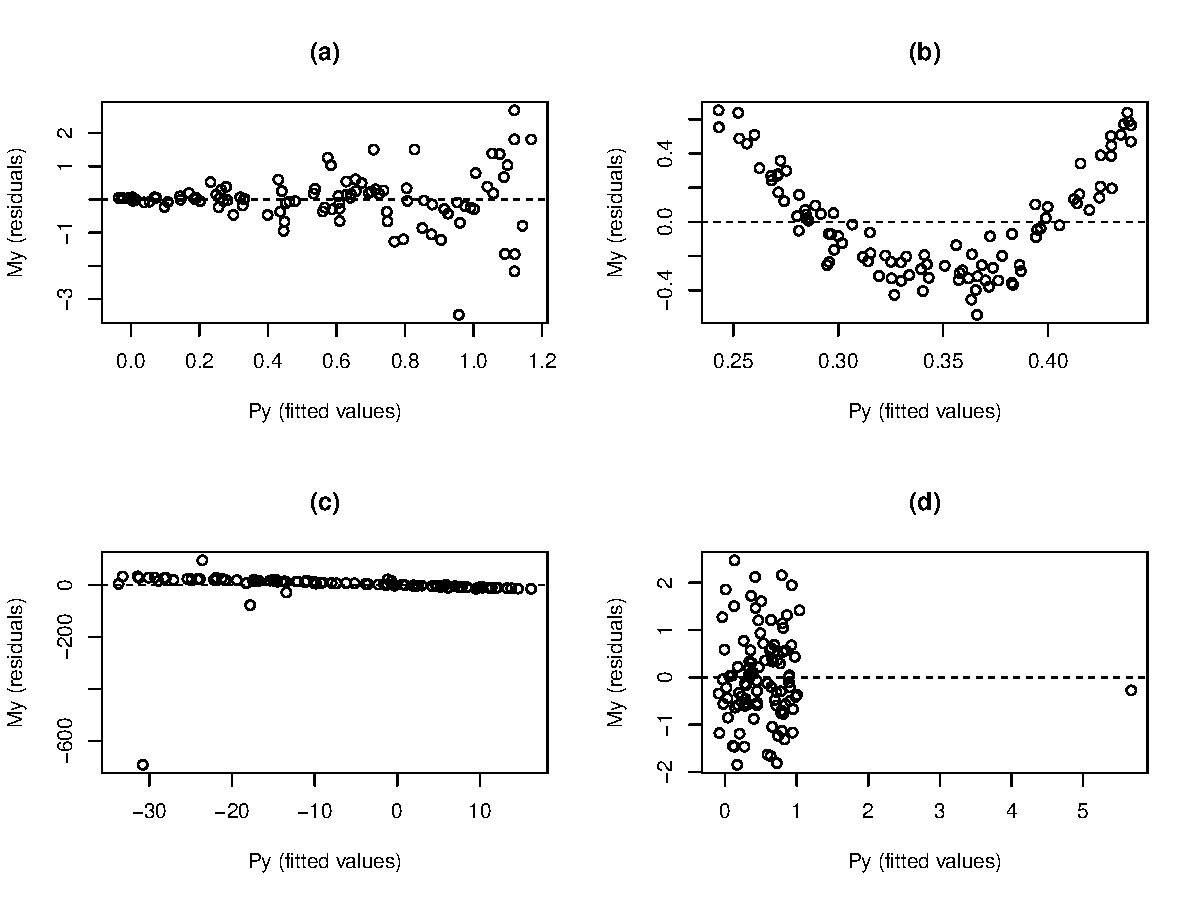
\includegraphics[width=\textwidth]{fig01.pdf}

{\bf 2.} Give a geometric interpretation of why the projection matrix and
annihilator matrix are idempotent ($P = P^2$ and $M = M^2$).

{\bf 3.} If $u_i \sim_{i.i.d.} \mathcal{N} (0, 1)$ for $i$ between $1$ and
$n$, what is the distribution of $u^t P u$ where $P$ is the projection matrix
of an $n$-by-$p$ matrix $X$.

{\bf 4.} Construct an example where strict exogeneity is violated but weak
exogeneity is not.

{\bf 5.} What is the conceptual difference between prediction intervals and
confidence intervals?

{\bf 6.} In what way is the Gauss-Markov theorem (BLUE) stronger than the
Cramér–Rao bound?

\end{document}





